\documentclass[12pt]{article}
\usepackage{xeCJK}

\usepackage{EngReport}


\graphicspath{{Images/}}
\bibliography{Sources}
\onehalfspacing
\graphicspath{{images/}}
\geometry{letterpaper, portrait, includeheadfoot=true, hmargin=1in, vmargin=1in}

%\fontsize{font size}{vertsize (usually 1.2x)}\selectfont

\begin{document}
\renewcommand{\familydefault}{\rmdefault}

\begin{titlepage}
    \begin{center}
    {\fontsize{40}{48}\selectfont \bfseries Multivariate Statistics} 
    \\\vspace{20pt}
    {\LARGE Final assigment} \\
    \vspace{20pt}
    \textbf{Daniel Alconchel, Mario García, Pablo Fuentes}
    \vspace{8pt}
    \\ \today
    \end{center}

    \bigskip
\begin{abstract}
In this project, we will analyze a database containing data on various aspects of residential homes in Ames, Iowa.

Our initial step involves a comprehensive exploratory data analysis to identify potential missing values and outliers. We will make decisions to address these issues.

Secondly, we will conduct a Principal Component Analysis (PCA). This technique aims to condense information from the original variables into a few linear combinations. The objective is to achieve dimensionality reduction while maximizing variance. These linear combinations are designed to be perpendicular to each other, aligning with the directions of maximum variance and ensuring lack of correlation.

Next, we will perform Factor Analysis (FA), identifying latent variables that exhibit a high correlation with specific groups of observable variables and minimal correlation with others. FA facilitates dimensionality reduction by capturing the underlying structure in the data.

In the final stage, we will execute both Linear Discriminant Analysis (LDA) and Quadratic Discriminant Analysis (QDA). Prior to these analyses, we will verify the necessary assumptions of normality. Discriminant Analysis is a classification method for qualitative variables. It allows the categorization of new observations based on their characteristics (explanatory or predictor variables) into different categories of the qualitative response variable
    \end{abstract}
\end{titlepage}
\pagestyle{fancy}
\fancyhf{}
\setlength{\headheight}{30pt}
\renewcommand{\headrulewidth}{0.4pt}
\renewcommand{\footrulewidth}{0.4pt}
\lhead{Multivariate Statistics}
\rhead{Daniel, Mario, Pablo}
\rfoot{\textbf{Page \thepage}}
\lfoot{}
\tableofcontents
\pagebreak



\pagebreak

% % % % % % % % % % % % % % % % % % % %
% % % % %  REPORT CONTENT   % % % % % %
% % % % % % % % % % % % % % % % % % % %

\fontsize{12}{20}\selectfont{
\section{Materials and methods}
\subsection{Materials}
In order to carry out the study we have taken a dataset from Kaggle. This dataset has information about multiple indicators about houses and more that 1000 observations. We have taken a subset of the variables of this set:
\begin{enumerate}
    \item \textbf{GrLivArea}: Above grade living area in square feet.
    \item \textbf{GarageArea}: Area of the garage in square feet.
    \item \textbf{1stFlrSF}: Area of the first floor in square feet.
    \item \textbf{OverallQual}: Rates the overall material and finish of the house.
    \item \textbf{LotArea}: Lot size in square feet.
    \item \textbf{YearBuilt}: Year of construction.
    \item \textbf{SalePrice}: The sale price of the house.
\end{enumerate}

Next we show a table with the basic descriptive statistics:
    %% Tabla aqui

    \begin{table}
        \centering
        \begin{tabular}{c|cccc}
        \hline
             & GrLivArea  & Garage Area & 1stFlrSF & LotArea  \\
             \hline
             Minumum & 334.0 & 0.0 & 334.0 &  1300.0 \\
             Q1 & 1129.0 & 333.0 & 882.0 &  7549.0 \\
             Median & 1464.0 & 480.0 & 1087.0 &  9478.5 \\
             Q3 & 1777.0 & 576.0 & 1391.5 &  11603.0 \\
             Maximum & 5642.0 & 1418.0 & 4692.0 &  215245.0 \\
             &  &  &  &   \\
             Mean & 1515.46 & 472.98 & 1162.63 & 10516.83  \\
             Std. Dev.& 52.485 & 213.80 & 386.59 &  9981.26 \\
             Coef. of variation & 0.35 & 0.45 & 0.33 & 0.95 \\
             &  &  &  &   \\
             Skewness& 1.36 & 0.18 & 1.37 &  12.18 \\
             Kurtosis & 4.86 & 0.9 & 5.71 &   202.26 \\
             \hline
        \end{tabular}
        \label{tab:table}
    \end{table}

    \begin{table}
        \centering
        \begin{tabular}{c|ccc}
             \hline
             &  OverallQual & YearBuilt & SalePrice \\
             \hline
             Minumum & 1 & 1872 &  34900.0 \\
             Q1 & 5 & 1954 & 129950  \\
             Median & 6 & 1973 & 163000  \\
             Q3 & 7 & 2000 & 214000  \\
             Maximum & 10 & 2010 & 755000  \\
             &  &  &   \\
             Mean & 6.1 & 1971 &  180921 \\
             Std. Dev.& 1.38 & 30 &  79442 \\
             Coef. of variation & 0.23 & 0.02 &  0.44 \\
             &  &  &  \\
             Skewness& 0.22 & -0.61 & 0.06  \\
             Kurtosis & 0.09 & -0.45 &  6.50 \\
             \hline
        \end{tabular}
        \label{tab:table}
    \end{table}
    
    \begin{table}
        \centering
        \begin{tabular}{cccc}
             &  &  & \\
             &  &  & \\
             &  &  & \\
             &  &  & \\
        \end{tabular}
        \caption{Caption}
        \label{tab:my_label}
    \end{table}
        
    \subsection{Statistical methods}
    We have carried out an exploratory analysis of the data in order to indetify missing values and/or outliers. First of all, we note that meanwhile out dataset does not have any missing data, it has outliers. For the outliers we made some boxplot graphics and replaced the outliers with the mean value of each variable after some analysis. We also repeated the procedure with normalized data in order to show a better visualization.

    Next, we made a classic numerical descriptive analysis showing some statistics such as the mean, std. deviation, median, etc. and some plots so we can understand better how the data behaves.

    In third place, we applied some techniques from multivariate analysis not without checking for the necessary requirement beforehand:

    \begin{enumerate}
        \item \textbf{Correlation between data}: At poblational level we made use of the Bartlett spherical constract and at sample level we used the correlation matrix and other useful graphical representations.
        \item \textbf{Univariate normality}: We made an exploration of the data through plots and histograms. This could give us an idea before hand, but we also made use of the Shapiro-Wilks normality test for checking the normality.
        \item \textbf{Multivariate normalit}y: We made use of the Royston test.
    \end{enumerate}

    Once all the requirements where checked (we ran into some problems which will be explained later in the results section) we applied some multivariate techniques. We made a \textbf{Principal Component Analysis} or \textbf{PCA} in order to reduce the dimensionality of the data through the observed data. Also a \textbf{Factorial Analysis} or \textbf{FA} was performed in order to indentify latent variables that would have high correlation with our observed variables. Finally, \textbf{Discriminant Analysis}, both linear and quadratic, and \textbf{Clustering} whas performed in order to find hidden patterns in our data.
\section{Results}
    First of all, no variable presented any kind of \textbf{missing data} so we skipped any treatment. In the case that we would have missing data we should analyze the data and checked the null hypothesis of homogenity. Second place, we decided to substitute the \textbf{outliers} with the means of the rest of the values.


    Next, the Bartlett test give us evidence to \textbf{reject} the hypothesis of independence, so some kind of \textbf{correlation existed} between the data and the we could perform a \textbf{Principal Component Analysis} and a \textbf{Factor Analysis}. By the \textbf{rule of Abdi} we got that we should choose \textbf{2 components}. In the Factor Analysis we made use of some plots and methods such as \textbf{Scree plot} and the \textbf{Elbow Method} and run a \textbf{maximum-likelihood factor analysis} test with the \textit{factanal} function chossing 3 factors.


    Next we show some plots showing the explained variance with de principal components and a diagram showing us the correlation of the latent variables:
    %% grafica varianza explicada pca
    \begin{figure}[h]
        \centering
        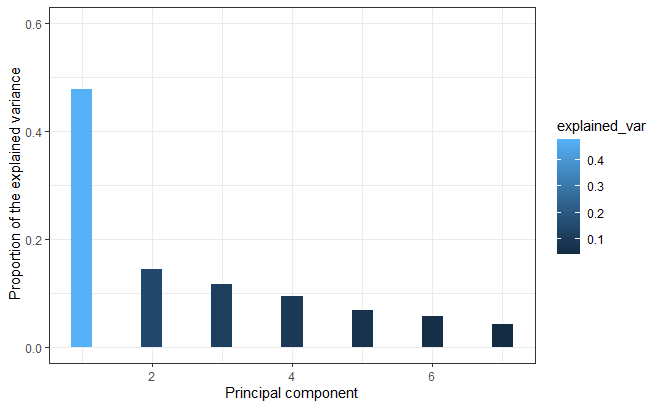
\includegraphics[width=0.5\textwidth]{varianza.png}
        \caption{Explained variance from the PCA}
        \label{fig:variance}
    \end{figure}
    %% Diagrama factor analysis
    \begin{figure}[h]
        \centering
        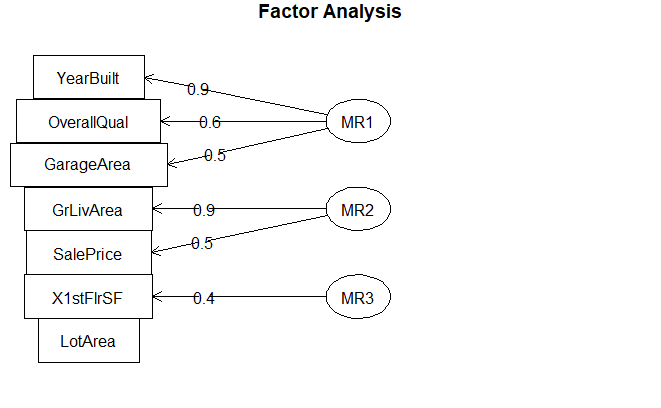
\includegraphics[width=0.5\textwidth]{diagrama.png}
        \caption{Diagram showing the correlations of the latent variables}
        \label{fig:diagram}
    \end{figure}

    
    Also defined a cathegoric variable through the sale price variable and we performed a \textbf{Discriminant Analysis} both Linear and Quadratic. We used the rest of the variables as predictors. In the case of the Linear Discrimant Analysis we obtain an error of 11.9\% and in the case of the Quadratic Discriminant Analysis we obtain an error of 12.39\%. Here we should note that our normality test, both of univariate and multivariate, told us to reject the hypothesis so we shouldn't be on conditions of applying this techniques. Even though, we decided to apply them but knowing beforehand that the performance could be worse that expected.


    Finally we performed a clustering analysis using both hierarchical (\textbf{Ward's method}) and non-hierarchical (\textbf{K-means}) methods. We used the \textbf{Siloutte method}, \textbf{WSS method} and \textbf{Gap Statistical} in order to estimate the optimal number of clusters for the K-Means methods. After analyzing the results we decided to stick with only 2 clusters.

    We are not showing any kind of graphic for this two last points since the high ammount of observations that we have makes them quite difficult to analyze. Still, one can refer to the \textit{RMarkdown} source code and see the corresponding plots for this parts.
    
\section{Discussion}
The data that we studied refered to 7 indicators for over 1000 houses. We studied the dimensionality reduction and stablish a method for classify these houses by these variables.

Through the correlation matrix we could see that all variables except \textit{LotArea} mantained a high correlation between them and this was reflected in the PCA since the first component explained all variables except \textit{LotArea} and the second one explained almost exclusively the former. 

The Factor analysis show us that 3 factors are enough to explain the data:
\begin{enumerate}
    \item The first latent variable correlates the year built, the overall quality and the garage area. We may understand this variable as the \textbf{quality of the house}. Makes sense to think that newer houses would have a better construction quality.
    \item The second one correlates the price and the total area of the house. One can think that the area of the house would be the factor that most determines the price of it.
    \item Finally we have a third variable that only correlates the area of the first floor, meaning that it does not share a lot with the other variables.
\end{enumerate}

We should note that no latent variable correlates the \textit{LotArea} which makes sense by looking before hand at our PCA.

We also decided to classify the data according to the price of the house into "high" and "low" so we can in the future determine the price of a house according to these indicators. We have performed the classification through both Lineal and Quadratic Discriminant Analysis.

Finally we decided to perform a Cluster Analysis in order to find hidden patterns into our data. In the clusters we seen that the mean values of the variables of each cluster are not similar except for \textit{LotArea} giving us another reason to think that it is not an interesting variable to take into account as an indicator for a house.
\section{Conclusion}
In this assigment we studied some indicators for multiple houses. We have explored the data, seeing that there is \textbf{no normality} into the data. We noted that the most important qualities for a house following this indicators can be summmarized as \textbf{the build quality} and the \textbf{the area of the house}. We concluded also that the \textit{LotArea} variable bring us almost no information. Finally we obtained a method for classifying the price of the houses according to this indicators allowing people in the real state market obtain better estimations for house prices.
}

\printbibliography

\end{document}
